%%%%%%%%%%%%%%%%%%%%%%%%%%%%%%%%%%%%%%%%%%%%%%%%%%%%%%%%%%%%%%%%%%%%%%%%%%%%%%%%
%2345678901234567890123456789012345678901234567890123456789012345678901234567890
%        1         2         3         4         5         6         7         8
%% main.tex
%% V1.0
%% 2017/02/22
%% by Francisco Maria Calisto
%% based on a template created by Rob Oakes
%%%%%%%%%%%%%%%%%%%%%%%%%%%%%%%%%%%%%%%%%%%%%%%%%%%%%%%%%%%%%%%%%%%%%%%%%%%%%%%%

\documentclass[a4paper,12pt]{texDoc}
% --> Please Choose the MAIN LANGUAGE for the document in package BABEL
% --> by replacing "main=" in language name selector. Default is "main=english"
\usepackage[main=english,portuguese]{babel} % Defines Main language
\usepackage[utf8]{inputenc}
\usepackage{iflang}
\usepackage{ifthen}
\usepackage{parskip}
\setlength{\parindent}{15pt}
\logo{
\includegraphics[width=0.3\textwidth]{IST_A_RGB_POS.png}} % Logo

%%%%%%%%%%%%%%%%%%%%%%%%%%%%%%%%%%%%%%%%%%%%%%%%%%%%%%%%%%%%%%%%%%%%%%%%%%%%%%%%
%	MEMO INFORMATION --> Write your info in the following tags.
%%%%%%%%%%%%%%%%%%%%%%%%%%%%%%%%%%%%%%%%%%%%%%%%%%%%%%%%%%%%%%%%%%%%%%%%%%%%%%%%

\docfrom{Francisco Maria Calisto} % Sender(s) Name
\docid{ist170916} % Student ID
\doccourse{AE 2016/2017} % Course Name, or abbreviated acronym
\docsubject{Problem Sheet \# 1 - Study} % Subject
\docdate{\today} % Date, -> set to \today for automatically print todays date

%%%%%%%%%%%%%%%%%%%%%%%%%%%%%%%%%%%%%%%%%%%%%%%%%%%%%%%%%%%%%%%%%%%%%%%%%%%%%%%%

\begin{document}
\maketitle % Print the doc header information

%%%%%%%%%%%%%%%%%%%%%%%%%%%%%%%%%%%%%%%%%%%%%%%%%%%%%%%%%%%%%%%%%%%%%%%%%%%%%%%%
%	LETTER CONTENT --> Your content is written here
%%%%%%%%%%%%%%%%%%%%%%%%%%%%%%%%%%%%%%%%%%%%%%%%%%%%%%%%%%%%%%%%%%%%%%%%%%%%%%%%

\section*{Question 1}

\subsection*{Answer}

R: b)

Why do I believe that I am correct?

b) The defined concepts and description of a system architecture and requirements for determine whether the description of an architecture conforms with are:

- Structural/Behavioural: behavioural concepts are the Assign to structural elements (assets) To indicate who or what offers certain behaviour.

- External/Internal: external or internal view of "systems".

- Individual/ Collective-Distinction: between behaviour executed by individual structural elements and collective behaviour performed by a collaboration of multiple structural elements.

\subsection*{Why the others are wrong?}

a) A representative enterprise architecture should be defined \cite{eaFundamentals} by three layers:

- Business: it offers services to customers through products, where the services are realized by business processes that use the informational entities of the organization and run by business actors.

- Application: supports the level of business with application services realized in application components.

- Technological: provides infrastructure services, like processing, storage and communication, to the application layer and it is where also the services are realized by software, machines and computer devices.

\begin{center}
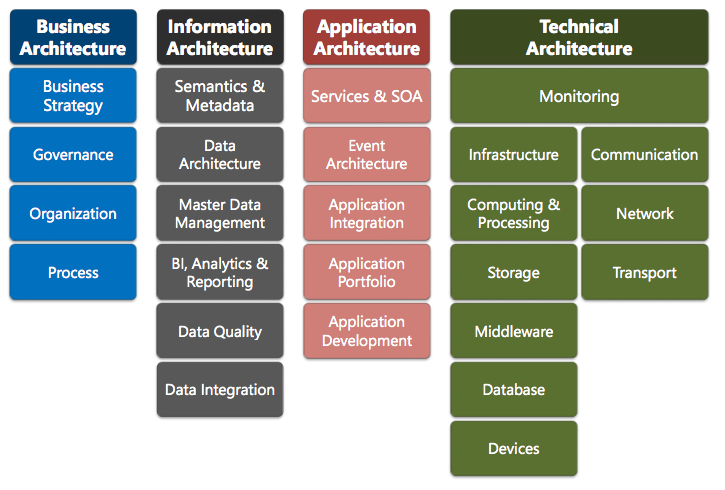
\includegraphics[width=0.75\textwidth]{concepts.png}
\end{center}

c) To establish concepts and methods, to identify and specify views and perspectives on the architecture, it may be relevant to distinguish between architecture principles that are relevant to:

- All employees of the organization.

- Employees of a specific part of the organization (business unit).

- Principles that are only relevant to employees in a specific role (e.g. software developers).

d) The standard focuses on the concepts of business process and stakeholder are:

\begin{center}
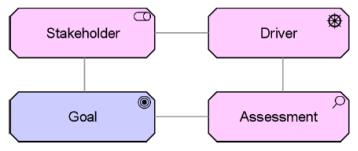
\includegraphics[width=0.75\textwidth]{stakeholders.png}
\end{center}

Since the stakeholder viewpoint focuses on modeling the stakeholders, drivers, the assessments of these drivers, and the initial goals to address these drivers and assessments.

\section*{Question 2}

Fundamentally a good philosophy abou the architecture is that it needs to be holistic, and that one should leverage best practices instead of developing everything from scratch. This philosophy has evolved from a repeated observation that managers who create a fragmented architecture practice that is not embedded into everyday corporate processes, and architects who ignore the great work that is already out there, are two common causes for failure of an architecture practice. On the other hand, Enterprise Architecture (EA) looks at the goals, opportunities and challenges facing the company, and seeks to propose solutions that can holistically improve the enterprise.

Everything must be on the right position to feed the right integration of the people who manage the requirements of every environments inside of an architecture. Those, are well seen in the next Figure:

\begin{center}
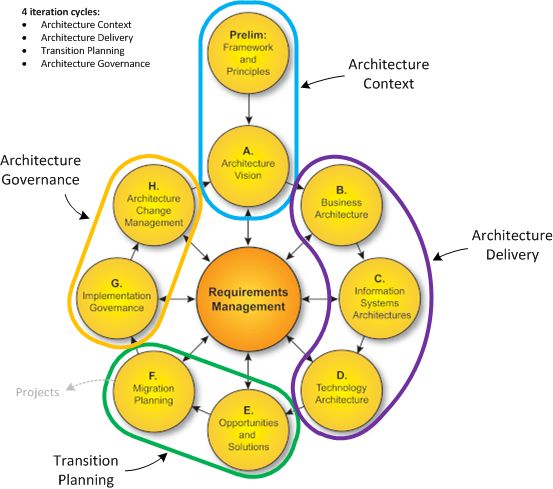
\includegraphics[width=0.75\textwidth]{togaf-adm.png}
\end{center}

In conclusion architecture in practice is a holistic endeavour of continuous improvement that is both broad and deep. Architecture Domains and Architecture Tiers are simply a way to overlay conceptual columns and rows against this broad topic to allow us to artificially subdivide it and get our heads around it.

\break


%%%%%%%%%%%%%%%%%%%%%%%%%%%%%%%%%%%%%%%%%%%%%%%%%%%%%%%%%%%%%%%%%%%%%%%%%%%%%%%%
%	DOCUMENT BIBLIOGRAPHY --> Your bibliography is written here
%%%%%%%%%%%%%%%%%%%%%%%%%%%%%%%%%%%%%%%%%%%%%%%%%%%%%%%%%%%%%%%%%%%%%%%%%%%%%%%%

\begin{thebibliography}{9}
\bibitem{eaFundamentals}  Enterprise Architecture Fundamentals. Available from World Wide Web: (AE\_fundamentals\_Fev\_2017\_v0\_8.pdf).
\bibitem{togaf-adm}  TOGAF-ADM: Architecture Principles. Available from World Wide Web: (http://pubs.opengroup.org/architecture/togaf9-doc/arch/chap23.html).
\end{thebibliography}

%%%%%%%%%%%%%%%%%%%%%%%%%%%%%%%%%%%%%%%%%%%%%%%%%%%%%%%%%%%%%%%%%%%%%%%%%%%%%%%%
\end{document}